\documentclass[a4paper, 11pt]{article}
\usepackage[margin=3cm]{geometry}
\usepackage[]{fontenc}
\usepackage[utf8]{inputenc}
\usepackage[italian]{babel}
\usepackage{geometry}
\geometry{a4paper, top=2cm, bottom=3cm, left=1.5cm, right=1.5cm, heightrounded, bindingoffset=5mm}
\usepackage{amsmath}
\usepackage{amssymb}
\usepackage{gensymb}
\usepackage{graphicx}
\usepackage{psfrag,amsmath,amsfonts,verbatim}
\usepackage{xcolor}
\usepackage{color,soul}
\usepackage{fancyhdr}
\usepackage{indentfirst}
\usepackage{graphicx}
\usepackage{newlfont}
\usepackage{amssymb}
\usepackage{amsmath}
\usepackage{latexsym}
\usepackage{amsthm}
%\usepackage{subfigure}
\usepackage{subcaption}
\usepackage{psfrag}
\usepackage{footnote}
\usepackage{graphics}
\usepackage{color}
\usepackage{hyperref}
\usepackage{tikz}
\usepackage{float}


\usetikzlibrary{snakes}
\usetikzlibrary{positioning}
\usetikzlibrary{shapes,arrows}

	
	\tikzstyle{block} = [draw, fill=white, rectangle, 
	minimum height=3em, minimum width=6em]
	\tikzstyle{sum} = [draw, fill=white, circle, node distance=1cm]
	\tikzstyle{input} = [coordinate]
	\tikzstyle{output} = [coordinate]
	\tikzstyle{pinstyle} = [pin edge={to-,thin,black}]

\newcommand{\courseacronym}{CAT}
\newcommand{\coursename}{Controlli Automatici - T}
\newcommand{\tipology}{A }
\newcommand{\trace}{3}
\newcommand{\projectname}{Controllo trattamento farmacologico su popolazioni cellulari}
\newcommand{\group}{21}

%opening
\title{ \vspace{-1in}
		\huge \strut \coursename \strut 
		\\
		\Large  \strut Progetto Tipologia \tipology  - Traccia \trace 
		\\
		\Large  \strut \projectname\strut
		\\
		\Large  \strut Gruppo \group\strut
		\vspace{-0.4cm}
}
\author{Barone Leonardo, Del Giudice Domenico, Galli Francesco, Guzzonato Leonardo}
\date{Gennaio 2025}

\begin{document}



\maketitle
\vspace{-0.5cm}

Il progetto riguarda l’utilizzo di tecniche di controlli automatici per il trattamento farmacologico di cellule in ambiente di laboratorio.\newline \newline
\textbf{Descrizione del problema} \newline \newline
Si consideri un gruppo di cellule in cui sono presenti una densità di cellule $n_s(t)$ suscettibili al trattamento farmacologico e una densità di cellule $n_r(t)$ resistenti. Si supponga che la loro evoluzione sia descritta dalle
seguenti equazioni differenziali

%
\begin{subequations}\label{eq:system}
\begin{align}
	\dot{n}_s=r_s \bigl(1-\frac{n_s+n_r }{K}\bigr)\, n_s\, -m_s\, c_f\, n_s\, -\beta\, n_s\, +\gamma\, n_r\, -\alpha\, c_f\, n_s\ ,
\end{align}
\begin{align}
	\dot{n}_r=r_r \bigl(1-\frac{n_s+n_r }{K}\bigr)\, n_r\, -m_r\, c_f\, n_r\, +\beta\, n_s\, -\gamma\, n_r\, +\alpha\, c_f\, n_s\ ,
\end{align}
\end{subequations}
%


dove i parametri $r_s, r_r \in \mathbb{R}$ rappresentano i tassi di riproduzione delle due tipologie, mentre il parametro $K \in \mathbb{R}$ rappresenta la densità massima di cellule che l’ambiente può contenere. La variabile d’ingresso $c_f(t)$ indica la concentrazione del farmaco. In particolare, i parametri $m_s, m_r \in \mathbb{R}$ determinano, rispettivamente, la mortalità delle cellule suscettibili e quella delle cellule resistenti, con $m_s > m_r$. Tipicamente, le cellule possono mutare da una tipologia all’altra. Ad esempio, le cellule suscettibili possono diventare resistenti, come tenuto in conto dai termini $-\beta n_s$ nella prima equazione e $\beta n_s$ nella seconda equazione, con $\beta \in \mathbb{R}$. Analogamente, accade per le cellule resistenti attraverso il termine $\gamma n_r$, con $\gamma \in \mathbb{R}$. Infine, il termine $\alpha c_f n_r$ tiene conto delle cellule suscettibili che mutano in resistenti a seguito del trattamento farmacologico. Uno schema esplicativo è riportato in Figura~\eqref{eq:system}. 

\begin{figure}[h!]
    \centering
    \includegraphics[width=0.7\linewidth]{Figura1.png}
    \caption{Schema del modello~\eqref{eq:system} in cui sono rappresentati i flussi delle cellule}
    \label{fig:enter-label}
\end{figure}

Si supponga di poter misurare in ogni istante la densità di cellule resistenti $n_r(t)$



\section{Rappresentazione in Forma di Stato e Linearizzazione del Sistema intorno ad una coppia di equilibrio}

Si riporta il sistema~\eqref{eq:system} nella seguente forma di stato
%
\begin{subequations}
\begin{align}\label{eq:state_form}
	\dot{x} &= f(x,u)
	\\
	y &= h(x,u).
\end{align}
\end{subequations}
%
Pertanto, si individua lo stato $x$, l'ingresso $u$ e l'uscita $y$ del sistema come segue 
%
\begin{align*}
	x := \begin{bmatrix}
		n_s
		\\
		n_r
	\end{bmatrix}, \quad u := \begin{bmatrix}c_f\end{bmatrix}, \quad y := \begin{bmatrix}n_r\end{bmatrix}.
\end{align*}
%
Coerentemente con questa scelta, si ricava dal sistema~\eqref{eq:system} la seguente espressione per le funzioni $f$ ed $h$
%
\begin{align*}
	f(x,u) &:=\begin{bmatrix}
		 r_s \bigl(1-\frac{x_1+x_2}{K}\bigr)\, x_1\, -m_s\, u\, x_1\, -\beta\, x_1\, +\gamma\, x_2\, -\alpha\, u\, x_1\ 
	\\
	r_r \bigl(1-\frac{x_1+x_2 }{K}\bigr)\, x_2\, -m_r\, u\, x_2\, +\beta\, x_1\, -\gamma\, x_2\, +\alpha\, u\, x_1\ 
	\end{bmatrix}
\end{align*}
\begin{align*}
	h(x,u) &:= x_2
\end{align*}
%
Una volta calcolate $f$ ed $h$ si esprime~\eqref{eq:system} nella seguente forma di stato
%
\begin{subequations}\label{eq:our_system_state_form}
\begin{align}
	\begin{bmatrix}
		\dot{x}_1
		\\
		\dot{x}_2
	\end{bmatrix} &= \begin{bmatrix}
	r_s \bigl(1-\frac{x_1+x_2}{K}\bigr)\, x_1\, -m_s\, u\, x_1\, -\beta\, x_1\, +\gamma\, x_2\, -\alpha\, u\, x_1\ 
	\\
	r_r \bigl(1-\frac{x_1+x_2 }{K}\bigr)\, x_2\, -m_r\, u\, x_2\, +\beta\, x_1\, -\gamma\, x_2\, +\alpha\, u\, x_1\ 
\end{bmatrix} \label{eq:state_form_1}
\end{align}
\begin{align}
	y &= x_2
\end{align}
\end{subequations}
%
Per trovare la coppia di equilibrio $(x_e, u_e)$ di \eqref{eq:our_system_state_form}x si risolve il seguente sistema di equazioni
%
\begin{align}
	\begin{cases}
		r_s \bigl(1-\frac{n_{s,e}+n_{r,e}}{K}\bigr)\, n_{s,e}\, -m_s\, u_e\, n_{s,e}\, -\beta\, n_{s,e}\, +\gamma\, n_{r,e}\, -\alpha\, u_e\, n_{s,e}\, =0
		\\
		r_r \bigl(1-\frac{n_{s,e}+n_{r,e}}{K}\bigr)\, n_{r,e}\, -m_r\, u_e\, n_{r,e}\, +\beta\, n_{s,e}\, -\gamma\, n_{r,e}\, +\alpha\, u_e\, n_{s,e}\, =0
	\end{cases}
\end{align}
%
dal quale, isolando la $u(t)$, si ottiene:
%
\begin{subequations}
\begin{align}
	u_1(t)=\frac{r_s \bigl(1-\frac{n_{s,e}+n_{r,e}}{K}\bigr)\, n_{s,e}\,-\beta n_{s,e}\,+\gamma n_{r,e}}{(m_s+\alpha)\,n_{s,e}} 
	\\
	u_2(t)=\frac{r_r \bigl(1-\frac{n_{s,e}+n_{r,e}}{K}\bigr)\, n_{r,e}\,+\beta n_{s,e}\,-\gamma n_{r,e}}{m_r\,n_{r,e}+\alpha\,n_{s,e}}
\end{align}
\end{subequations}
%
calcolando quindi rispetto ai parametri forniti si ottiene
%
\begin{align}
	x_e :=\begin{bmatrix}
		n_{s,e}
		\\
		n_{r,e}
	\end{bmatrix} = 
	\begin{bmatrix}
		100
		\\
		400
	\end{bmatrix},  \quad u_e = 0 \
	\label{eq:equilibirum_pair}
\end{align}
%
Si definiscono le variabili alle variazioni $\delta x$, $\delta u$ e $\delta y$ come 
%
\begin{align*}
	\delta x \approx x(t)-x_e, \\
	\quad 
	\delta u = u(t)-u_e, \\
	\quad
	\delta y \approx y(t)-y_e. 
\end{align*}
%
L’evoluzione del sistema, espressa in termini delle variazioni delle variabili, può essere approssimativamente rappresentata attraverso il seguente sistema lineare.
%
\begin{subequations}\label{eq:linearized_system}
\begin{align}
	\delta \dot{x} &= A\delta x + B\delta u
	\\
	\delta y &= C\delta x + D\delta u,
\end{align}
\end{subequations}
%
con opportune matrici $A$, $B$, $C$ e $D$  calcolate nel seguente modo:
%
\begin{subequations}\label{eq:matrices}
\begin{align}
	A &= \begin{bmatrix}
		\frac{\partial}{\partial\,x_1}\,f_1(x,u)\bigg|_{x_e,u_e} & \frac{\partial}{\partial\,x_2}\,f_1(x,u)\bigg|_{x_e,u_e}
		\\
		\frac{\partial}{\partial\,x_1}\,f_2(x,u)\bigg|_{x_e,u_e} & \frac{\partial}{\partial\,x_2}\,f_2(x,u)\bigg|_{x_e,u_e}
	\end{bmatrix} 
	= 
	 \\ &= \begin{bmatrix}
r_s \left(1 - \frac{2x_1 + x_2}{K} \right) - m_s u_e - \beta - \alpha u_e  & \frac{r_s x_1}{K} + \gamma
		\\
\frac{r_r x_2}{K} + \beta + \alpha u_e & r_r \left( 1 - \frac{x_1+2x_2}{K} \right) - m_r u_e - \gamma
\end{bmatrix}
	=
	\begin{bmatrix}
		-1.14 & 0.54
		\\
		1.92 & -1.32
	\end{bmatrix}
	\\ \\ 
	B &= \begin{bmatrix}
		\frac{\partial}{\partial\,u}\,f_1(x,u)\bigg|_{x_e,u_e}
		\\
		\frac{\partial}{\partial\,u}\,f_2(x,u)\bigg|_{x_e,u_e}
	\end{bmatrix}
	=
	\begin{bmatrix}
		-m_s\,x_1-\alpha\,x_1
		\\
		-m_r\,x_2+\alpha\,x_1
	\end{bmatrix}
	=
	\begin{bmatrix}
		-145
		\\
		30
	\end{bmatrix}
	\\ \\
	C &= \begin{bmatrix}
		\frac{\partial}{\partial\,x_1}\,h(x,u)\bigg|_{x_e,u_e} & \frac{\partial}{\partial\,x_2}\,h(x,u)\bigg|_{x_e,u_e}
	\end{bmatrix}
	=\begin{bmatrix}
		0 & 1
	\end{bmatrix}
	\\ \\
	D &= \begin{bmatrix}
		\frac{\partial}{\partial\,u}\,h(x,u)\bigg|_{x_e,u_e}
	\end{bmatrix}
	= \begin{bmatrix}
	0
\end{bmatrix}
\end{align}
\end{subequations}
%
\begin{figure}[h!]
    \centering
    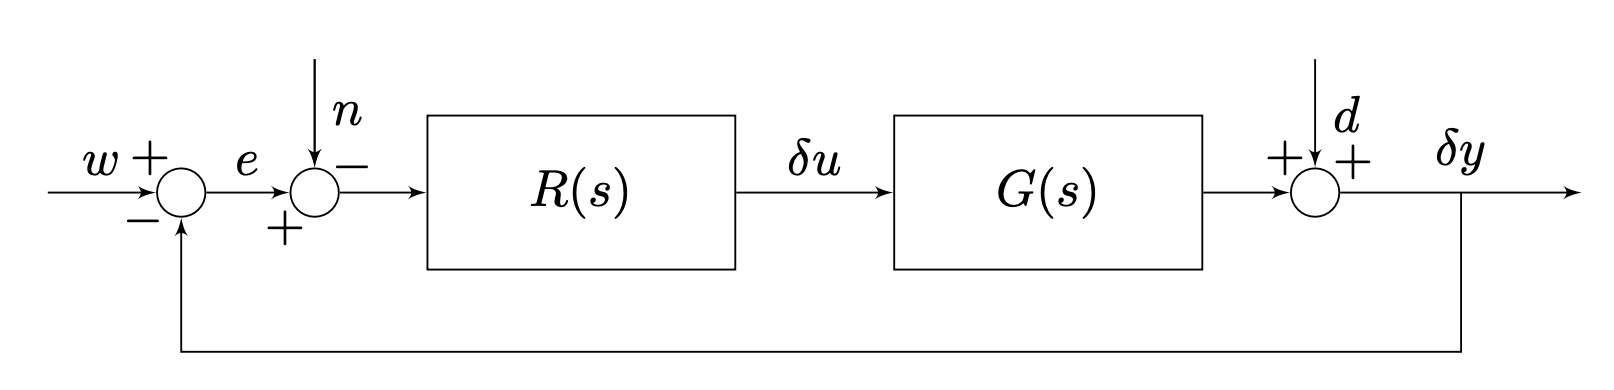
\includegraphics[width=0.7\linewidth]{Figura2.png}
    \caption{Schema di controllo~\eqref{figura2}}
    \label{figura2}
\end{figure}
\\ \\ \\ \\ \\ \\ \\ \\ \\ \\ \\ \\ \\ \\ 
\section{Calcolo Funzione di Trasferimento}

In questa sezione, si calcola la funzione di trasferimento $G(s)$ dall'ingresso $\delta u$ all'uscita $\delta y$ mediante la seguente formula 
%
%
\begin{align}\label{eq:transfer_function}
G(s) = C(sI-A)^{-1}B-D = -521.7869\ \frac{-0.1229s+1}{(0.444s+1)(4.812s+1)}.
\end{align}
%
Dunque il sistema linearizzato~\eqref{eq:linearized_system} è caratterizzato dalla funzione di trasferimento~\eqref{eq:transfer_function} con 2 poli \\ $p_1 = -0.2078,  p_2=-2.2522$ e uno zero $z = 8.14$. In Figura \eqref{bodediagram} si mostra il corrispondente diagramma di Bode. 

\begin{figure}[h!]
    \centering
    \includegraphics[width=0.7\linewidth]{BodeG.png}
    \caption{Diagramma di Bode della funzione di trasferimento G(s)}
    \label{bodediagram}
\end{figure}


\section{Mappatura specifiche del regolatore}
\label{sec:specifications}

Le specifiche da soddisfare sono:
\begin{itemize}
	\item[1)] L'errore a regime in risposta ad un segnale gradino $1(t)$ sia nullo\label{spec1}
	\item[2)] Il margine di fase $M_f\ge40^{\circ}$ per garantire robustezza al sistema\label{spec2}
	\item[3)] La sovraelongazione percentuale massima $S\%\ge7\%$\label{spec3}
	\item[4)] Il tempo di assestamento al $5\%$ inferiore a $1s$\label{spec4}
	\item[5)] Il disturbo in uscita $d(t)$ risulti attenuato di 60dB sapendo che la sua banda si limita a pulsazioni nel range $[0;0.05]$\label{spec5}
	\item[6)] Il disturbo di misura $n(t)$ risulti attenuato di 90dB sapendo che la sua banda si limita a pulsazioni nel range $[10^4;10^6]$\label{spec6}
\end{itemize}
%
Si effettua la mappatura punto per punto le specifiche richieste. 
\begin{itemize}
	\item[1)] Per azzerare l'errore a regime in risposta ad un segnale a gradino si inserirà un polo nell'origine durante la sintesi del regolatore statico\
	\item[2)] In corrispondenza della pulsazione critica $\omega_c$ si deve avere una fase maggiore di $-140^{\circ}$\
	\item[3)] Per ottenere una sovraelongazione percentuale massima $S\%\ge7\%$ poniamo $\xi=\frac{M_f}{100}$.
	\\
	Sapendo che la sovraelongazione massima e la $\xi$ massima rispettano la seguente relazione:\\
	 $S^\star=e^\frac{-\pi\xi^\star}{\sqrt{1-(\xi^\star)^2}}$.
	 \\
	 Sostituendo $\xi$ otteniamo $M_f\ge64,6^{\circ}$.
	\item[4)] Per ottenere un tempo di assestamento al $5\%$ inferiore a $1s$ è necessario imporre $e^{-\xi\omega_c\,T_a}=0.05$.\\
	Si ottiene quindi $\xi\omega_c\ge\frac{3}{T^\star}$ con $T^\star$ tempo di assestamento massimo.\\
	Da ciò si ricava quindi $\omega_c=\frac{300}{T^\star\,M_f}=4.644\frac{rad}{s}$.
	\item[5)] Per riuscire ad attenuare il disturbo in uscita $d(t)$ di 60dB risulta necessario che nell'intervallo d'interesse($[0;0.05]$) $|L(j\omega)|_{dB}\ge60dB$.\
	\item[6)] Per riuscire ad attenuare il disturbo di misura $n(t)$ di 90dB risulta necessario che nell'intervallo d'interesse($[10^4;10^6]$) $|L(j\omega)|_{dB}\le-60dB$.\
\end{itemize}
Pertanto, in Figura \ref{Figura 2}, si mostra il diagramma di Bode della funzione di trasferimento $G(s)$ con le zone proibite emerse dalla mappatura delle specifiche.

\begin{figure}[h]
	\centering
	\includegraphics[width=12cm]{GGconPatch}
	\caption[]{Diagramma di Bode di G(s) con patch delle zone proibite}
	\label{Figura 2}
\end{figure}

\section{Sintesi del regolatore statico}
\label{sec:static_regulator}


In questa sezione si progetta il regolatore statico $R_s(s)$ partendo dalle analisi fatte in sezione~\ref{sec:specifications}.\\
La progettazione del regolatore statico è volta alla risoluzione delle problematiche dovute alle specifiche $1$ e $5$ viste nel punto precedente.\\
Per ottenere errore a regime nullo in risposta al riferimento a gradino inseriamo un polo nell'origine. Si considera inoltre un guadagno statico del nostro regolatore $\mu_s=200$ per ottenere l'attenuazione richiesta di 60dB sul disturbo in uscita $d(t)$ a basse pulsazioni.
\\
\\
Il regolatore statico così sintetizzato risulta essere nella forma $R_s(s)=\frac{200}{s}$.\\
\\
Dunque, si definisce la funzione estesa $G_e(s) = R_s(s)G(s)$ e, in Figura \ref{Figura 3}, mostrando il suo diagramma di Bode per verificare se e quali zone proibite vengono attraversate.

\begin{figure}[H]
	\centering
	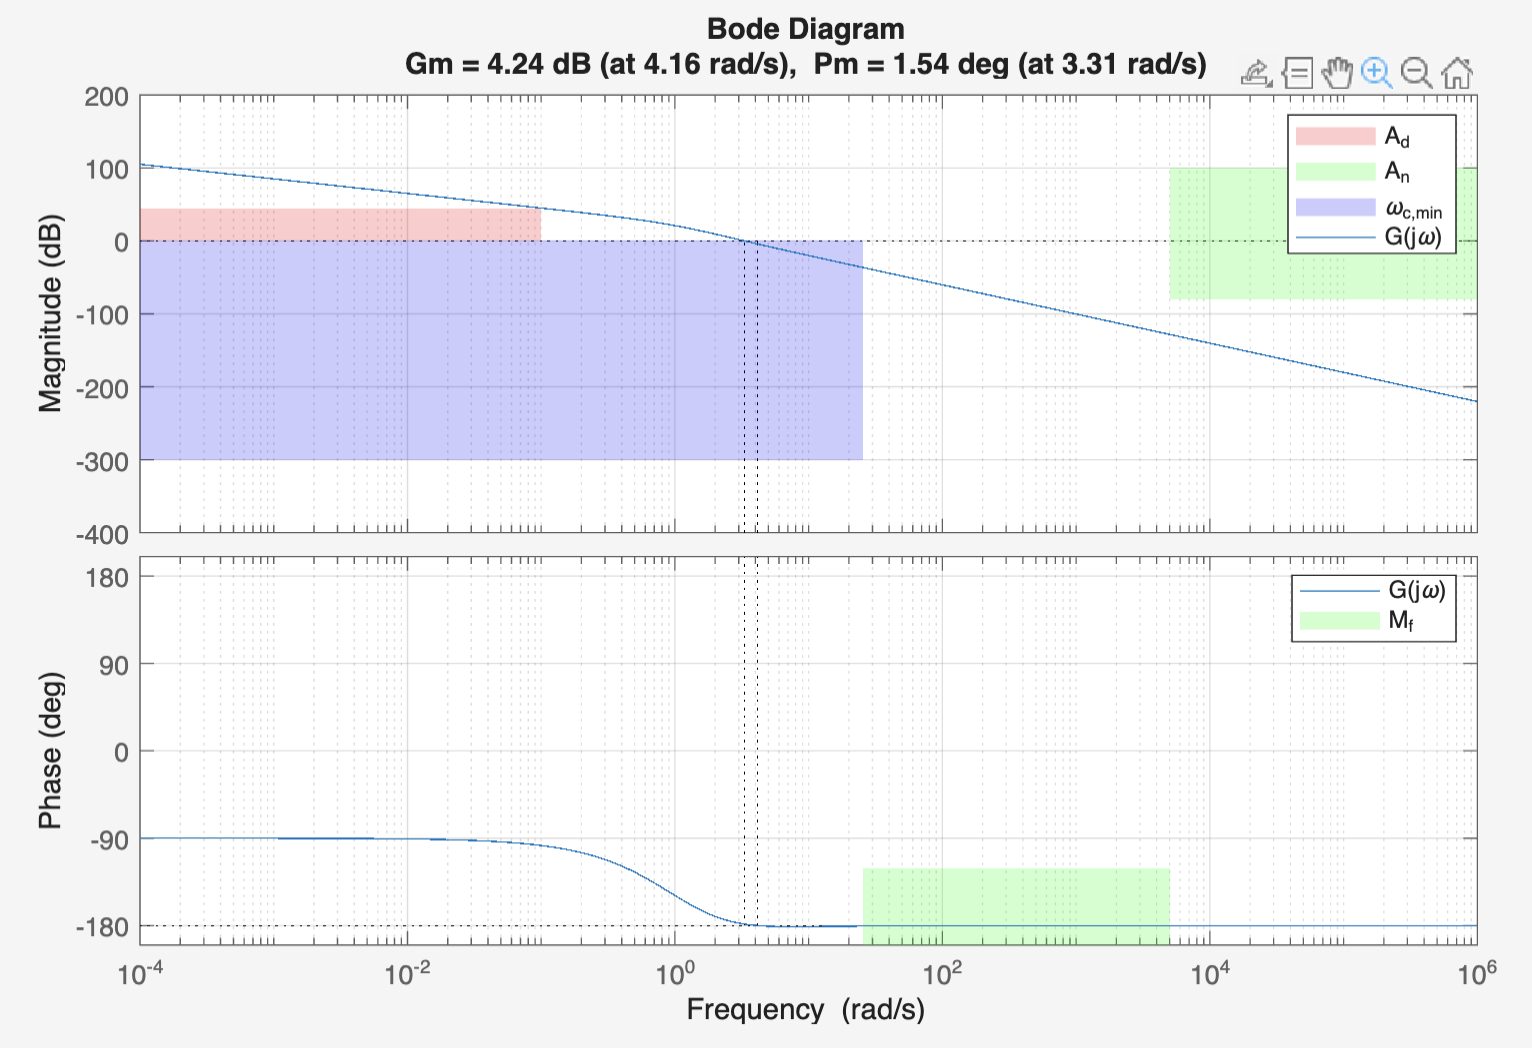
\includegraphics[width=12cm]{GeConPatch}
	\caption[]{Diagramma di Bode del sistema esteso con patch delle zone proibite}
	\label{Figura 3}
\end{figure}


Da Figura \ref{Figura 3} si può osservare che le specifiche riguardanti disturbo di misura $n(t)$ risultano essere rispettate, ma la fase del sistema esteso, dopo un crollo che supera i $-180^{\circ}$, risulta essere negativa nella pulsazione critica (pulsazione di attraversamento dello 0 nel diagramma dell'ampiezza).\\
Ciò non rispetta il teorema di Bode, il cui enunciato dice che, rispettate le ipotesi riguardo l'attraversamento dello 0 in un solo punto e la mancanza di poli a parte reale positiva (ipotesi rispettate dal nostro sistema), condizione necessaria e sufficiente per la stabilità di un sistema retroazionato è che la sua $L(j\omega)$ (in questo caso la nostra $G_e(s)$) risulti avere fase maggiore di $-180^{\circ}$ alla pulsazione critica $\omega_c$.
Dunque il sistema non solo non rispetta le specifiche riguardo a sovraelongazione e margine di fase, ma risulta essere addirittura instabile ed è quindi necessario risollevare la fase, operazione che verrà effettuata nella sintesi del regolatore dinamico.  

\section{Sintesi del regolatore dinamico}

In questa sezione, si progetta il regolatore dinamico $R_d(s)$. 
%
Dalle analisi fatte in Sezione~\ref{sec:static_regulator}, si nota di essere nello Scenario di tipo B, in cui tutto l'intervallo d'interesse per la nostra $\omega_c$ risulta avere fase minore di $-115.4^{\circ}$($-180^{\circ}+M_f$). Procediamo dunque alla progettazione del regolatore dinamico $R_d(s)$.
\\
Osservando l'andamento della $G(s)$ si può notare che l'andamento del diagramma della fase risulta essere estremamente vicino al rispetto delle specifiche. Pertanto si è scelto di inserire uno zero a basse frequenze all'interno del regolatore dinamico $R_d(s)$ ottenendo così la forma $R_d(s)=(1+5s)$.
\\
\\
In Figura \ref{Figura 4}, si osserva il diagramma di Bode della funzione dopo l'inserimento di uno zero a basse frequenze ($\omega_z=0.2$ $rad/s$).

\begin{figure}[H]
	\centering
	\includegraphics[width=12cm]{G_zeroConPatch}
	\caption[]{Diagramma di Bode del sistema esteso dopo l'inserimento dello zero}
	\label{Figura 4}
\end{figure}

Dal diagramma così ottenuto si può osservare come il sistema non rispetti ora la specifica riguardo l'attenuazione dei disturbi di misura $n(t)$ ad alte frequenze.
\\
Per ovviare a questo problema si inseriscono più poli ad alte frequenze. L'espressione del regolatore dinamico $R_d(s)$ risulta quindi essere $R_d(s)=\frac{(1+5s)}{(1+\frac{1}{2000}s)^4}$ .
\\

In Figura \ref{Figura 5}, si mostra il diagramma di Bode della funzione d'anello $L(s) = R_d(s) G_e(s)$

\begin{figure}[H]
	\centering
	\includegraphics[width=12cm]{LLconPatch}
	\caption[]{Diagramma di Bode del sistema esteso con regolatore dinamico completo}
	\label{Figura 5}
\end{figure}

Dopo la sintetizzazione del regolatore dinamico il sistema risulta essere correttamente regolato.
\section{Test sul sistema linearizzato}
\label{sec:testsistemalinearizzato}

In questa sezione, si testa l'efficacia del controllore progettato sul sistema linearizzato in risposta a segnali $w(t)=-2\cdot1(t)$, $d(t)=\sum_{k=1}^{4}0.3sin(0.0125kt)$ e $n(t)=\sum_{k=1}^{4}0.2sin(10^4kt)$.
\\
\\
Dopo aver ricavato le funzioni di sensitività $F(s)$ e $S(s)$ si analizza la risposta del sistema al segnale a gradino $w(t)$ (in Figura \ref{Figura 6}), al disturbo $d(t)$ (in Figura \ref{Figura 7}) e al disturbo $n(t)$ (in Figura \ref{Figura 8}) singolarmente.  
\\
\begin{figure}[H]
	\centering
	\includegraphics[width=12cm]{RispostaAGradino}
	\caption[]{Risposta al gradino con vincoli di sovraelongazione e tempo di assestamento evidenziati}
	\label{Figura 6}
\end{figure}
\begin{figure}[H]
	\centering
	\includegraphics[width=12cm]{RispostaAd(t)}
	\caption[]{Risposta al disturbo $d(t)$}
	\label{Figura 7}
\end{figure}
\begin{figure}[H]
	\centering
	\includegraphics[width=12cm]{RispostaAn(t)}
	\caption[]{Risposta al disturbo $n(t)$}
	\label{Figura 8}
\end{figure}

Si osserva che $y_w(t)$ rispetta pienamente le specifiche, inoltre $y_d(t)$ e $y_n(t)$ risultano essere attenuati in accordo ai requisiti.
\\
Si procede ora a sommare le tre risposte per ottenere il grafico della risposta complessiva del sistema (In Figura \ref{Figura 9}).\\
\begin{figure}[H]
	\centering
	\includegraphics[width=12cm]{RispostaComplessiva}
	\caption[]{Risposta complessiva $y(t)$}
	\label{Figura 9}
\end{figure}
\section{Test sul sistema non lineare}

In questa sezione si testa l'efficacia del controllore progettato sul modello non lineare in riferimento ai segnali visti nella Sezione \ref{sec:testsistemalinearizzato}.
\\
Per effettuare i test si è utilizzato l'ambiente Simulink offerto da Matlab.
Si è realizzato un modello di sistema in retroazione così strutturato.
\begin{figure}[H]
	\centering
	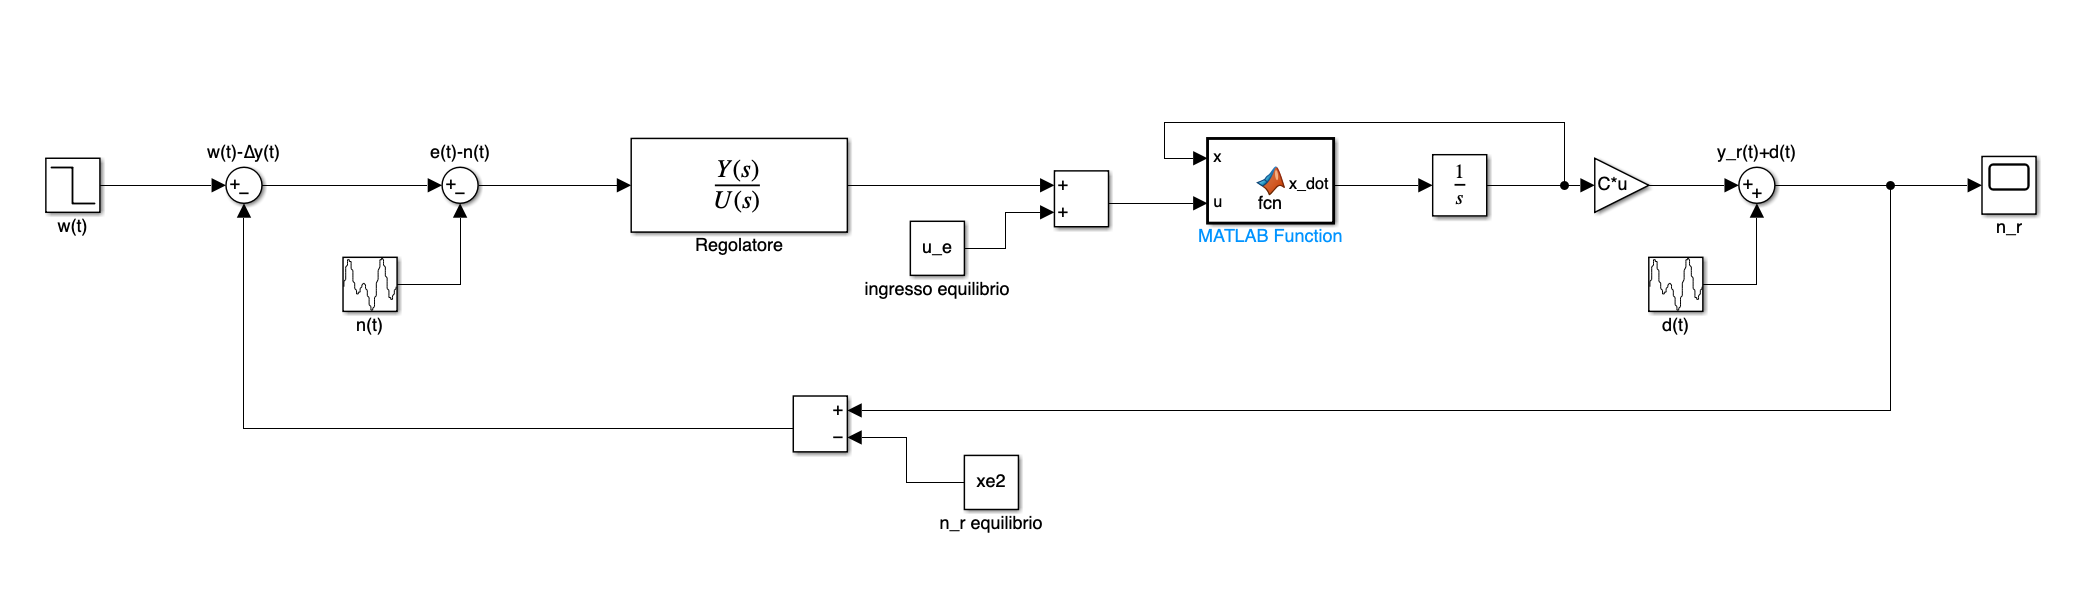
\includegraphics[width=15cm]{SistemaNonLineare}
	\caption[]{Risposta complessiva $y(t)$}
	\label{Figura 10}
\end{figure}

Nel caso di test riportato vengono considerati condizioni iniziali $x_0=\begin{bmatrix}
	95
	\\
	102
\end{bmatrix}$, il cui risultato è visibile in Figura \ref{Figura 11}
\begin{figure}[H]
	\centering
	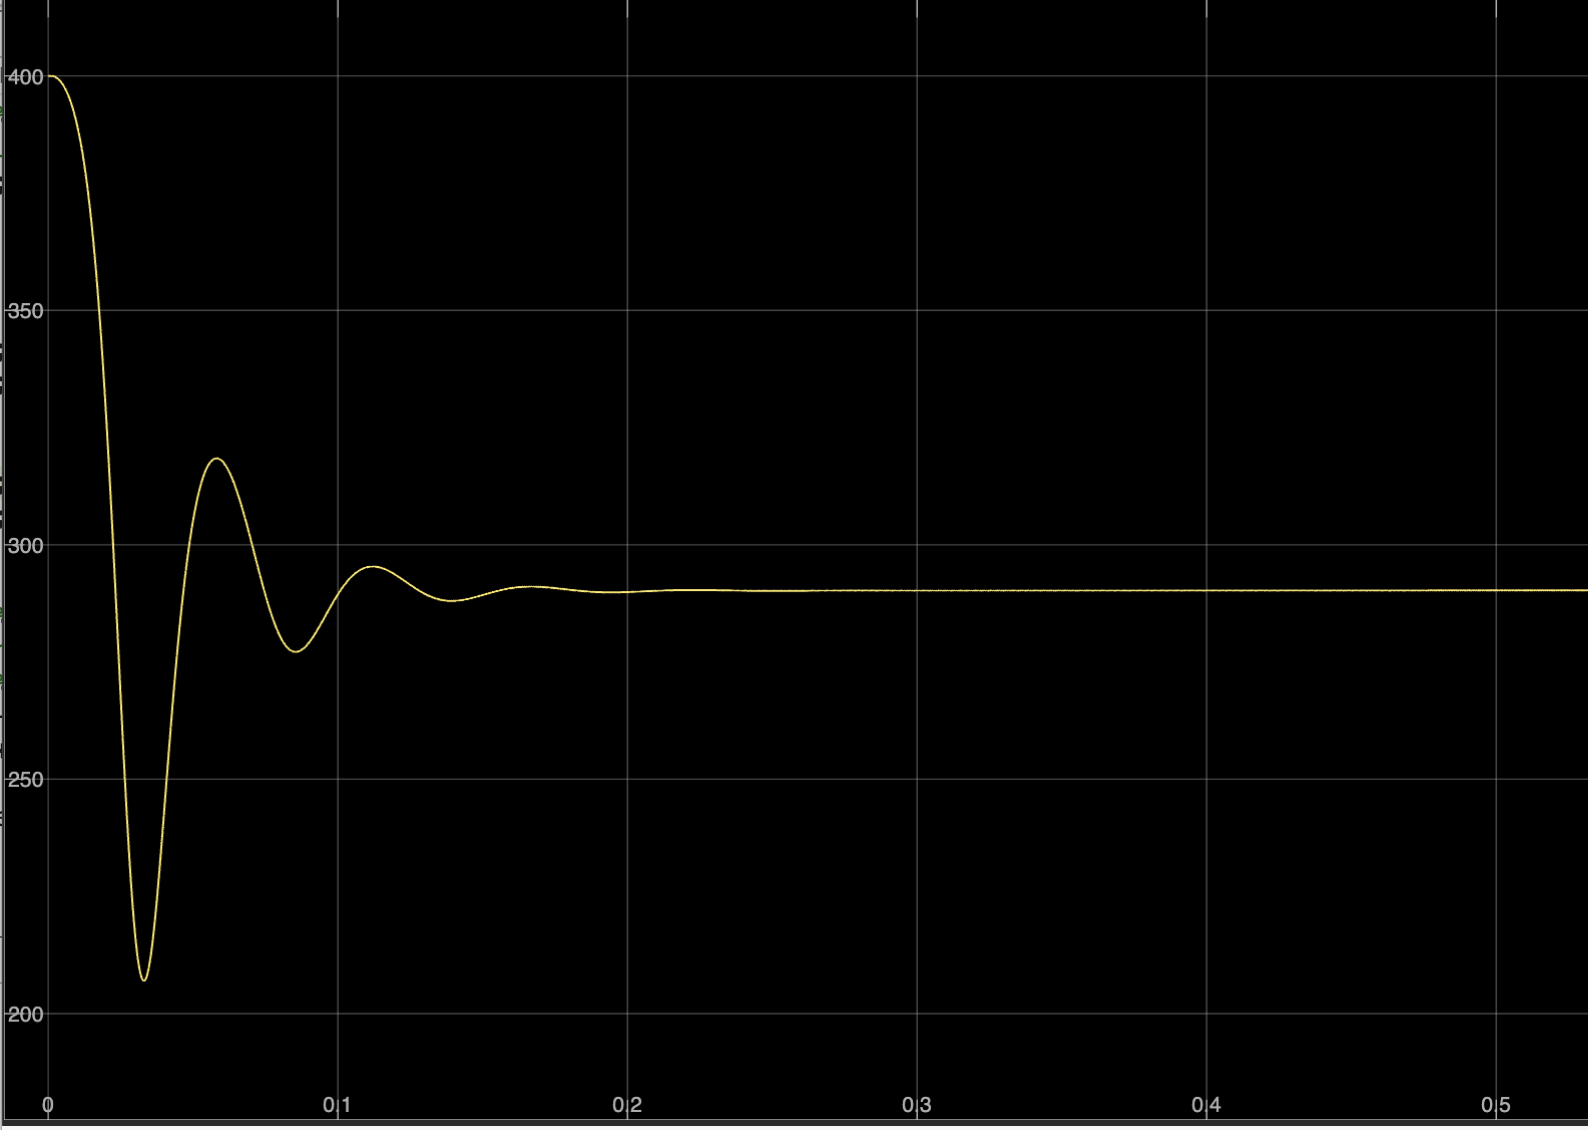
\includegraphics[width=12cm]{TestSistemaNonLinearizzato}
	\caption[]{Test del regolatore sul sistema non lineare}
	\label{Figura 11}
\end{figure}

A seguito dei test effettuati il sistema può dirsi stabile e regolato in accordo con le specifiche fornite, risulta inoltre possibile modificare le condizioni iniziali per testare altri casi, nei punti successivi si analizzerà la stabilità del sistema regolato allontanandosi dall'equilibrio e con vari riferimenti $w(t)$.
\section{Punti opzionali}
Al fine di ottenere i risultati in seguito riportati è stato utilizzato il modello realizzato su Simulink registrando gli output per realizzare l'interfaccia grafica e modificando condizioni iniziali ed ampiezza del gradino di riferimento su Matlab e osservando i risultati sul modello.

\subsection{Primo punto}

Per visualizzare l'andamento del numero di cellule all'interno della coltura si è scelto di utilizzare un diagramma a barre. L'applicazione utilizza il modello Simulink apportando una leggera modifica in modo che i valori di $n_s$ e $n_r$ siano visibili nel workspace. Impostando le condizioni iniziali tramite comando Matlab, avendo cura di aprire il progetto Simulink correlato, si può avviare la simulazione che mostra un'animazione dei diagrammi al trascorrere del tempo.

\subsection{Secondo punto}
Si analizza in questo punto la stabilità del sistema al variare delle condizioni iniziali posto il riferimento a 0 (non distanziandosi quindi dal punto di equilibrio).
Nel grafico riportato in Figura \ref{Figura 12} vengono evidenziate i range di condizioni iniziali (con precisione approssimata a valori interi in un piccolo intorno dell'equilibrio e a multipli di 5 successivamente). In rosso sono evidenziate le coordinate delle condizioni iniziali che non portano alla stabilità, in grigio la zona non considerata a causa della specifica sul numero massimo di cellule della coltura, in verde le coordinate che mantengono stabile il sistema e le zone bianche sono zone di transizione, in cui non sono stati effettuati test accurati.
\\
 \begin{figure}[H]
 	\centering
 	\includegraphics[width=12cm]{RangeCondInit}
 	\caption[]{Tabella dei valori validi del riferimento a gradino}
 	\label{Figura 12}
 \end{figure}


\subsection{Terzo punto}

In questo punto si analizza la stabilità del sistema al variare dell'ampiezza del riferimento a gradino.
\\
Viene di seguito riportata (Figura \ref{Figura 13}) una tabella con i valori per i quali il sistema si mantiene stabile. 
\begin{figure}[H]
	\centering
	\includegraphics[width=12cm]{TabellaValoriGradino}
	\caption[]{Tabella dei valori validi del riferimento a gradino}
	\label{Figura 13}
\end{figure}
\section{Conclusioni}

Durante il progetto si è realizzato un regolatore che permette il controllo del numero di cellule cancerose resistenti ad un determinato farmaco. Il riferimento considerato risulta essere relativo all'equilibrio; ciò è dovuto alla necessità di linearizzare il sistema per la progettazione del regolatore $R(s)$, questo causa una relativizzazione rispetto all'equilibrio preso in considerazione.
\\
Esplorando il range di condizioni iniziali possibili è possibile osservare come la diminuzione delle cellule sensibili non risulti particolarmente rilevante rispetto alla stabilità del sistema, contrariamente a quella delle cellule resistenti. Questo comportamento può essere spiegato tenendo in considerazione che il sistema utilizza come unico parametro in retroazione il numero di cellule resistenti presenti nella coltura.
\\
Si può osservare anche che è possibile aumentare significativamente il numero di cellule resistenti iniziali, aumento che viene limitato dal numero di cellule sensibili presenti.
\\
Esplorando il range del riferimento a gradino si osserva come il sistema rimanga stabile imponendo una riduzione delle cellule resistenti rispetto all'equilibrio, mentre imponendo un aumento il sistema diventa rapidamente instabile.
\\
\\
Come considerazione finale si noti inoltre che tutti i range presi in analisi astraggono notevolmente il problema, infatti si è tenuto conto solamente del raggiungimento del riferimento a regime, trascurando fattori imprescindibili nello studio del caso reale, quali una concentrazione negativa di farmaco (fisicamente non ottenibile) o un numero negativo di cellule in un istante di tempo (anch'esso privo di significato in un contesto reale).

\end{document}

